\section{TCP: Principles and practice}
\subsection{TCP headers}
\textbf{Part 1}\\
\begin{enumerate}
\item The purpose of the RST bit is to reset a connection. It is used
  when a client (or server) sends an invalid TCP segment. If for instance a
  client sends a SYN, receives a SYN-ACK, and then sends another SYN, the server
  will most likely send a RST packet.
\item The sequence number is sent with each segment of data. The first octet in
  the segment has a sequence number, which represents the segments sequence
  number. The acknowledgment number is part of the sequence number, and is used
  to identify the next expected octet.\\
  There is a relation between the sender and the receiver, otherwise the data
  sent could be arbitrary rubble.
\item The TCP window is used to indicate how much data the receiver is
  ready/willing to receive from the sender. A positive window size tells how
  many bytes the receivers buffer is able to hold.
\item The sender starts a timer and waits a certain amount of time, before
  sending a new package. The ACK from the receiver to the sender, should then
  contain a new window size, which is able to hold the data that the sender
  wants to send.
\end{enumerate}

\noindent \textbf{Part 2}
The client is able to send data to the server after receiving the sequence and
acknowledgment numbers with the SYN-ACK packet.\\

\noindent \textbf{Part 3}
\begin{figure}[h!]
  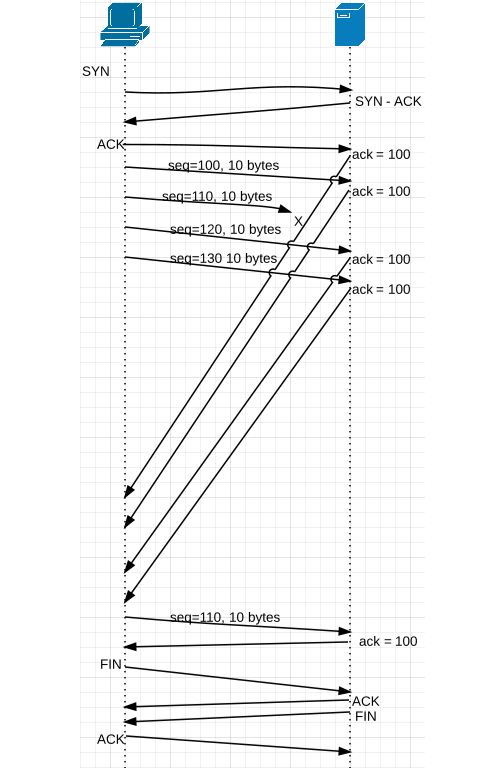
\includegraphics[scale=0.5]{tcpstuff.png}
\end{figure}
\newpage
\subsection{High performance TCP}
\begin{enumerate}
\item The maximum value is 64 KB, because the maximum size of a TCP packet is
    64 KB. It takes a lot of packages to send large files with such a small
    size.
\item First we calculate the maximum amount of bytes we can push out on the
    link
    \[
        \frac{100\cdot 10^6}{8} = 12.5 \cdot 10^6 B/s
    \]
    Then we calculate the maximum buffer size (64 KB) to bytes
    \[
        64 \cdot 10^6 B
    \]
    Note that we have not used powers of 2. Now we can calculate the RTT with
    \[
        \frac{64 \cdot 10^3 B}{12.5 \cdot 10^6 B/s} = 0.00512 s
    \]
    So the RTT is approximately 5 ms
\item FEEDBACK WANTED: Should we isolate the number of bytes from the above
    equation, or should we use the "shift.cnt" variable to define the amount of bytes?
\end{enumerate}

\subsection{Flow and Congestion Control}
\textbf{Part 1}\\
Modern TCP implements congestion control with the algorithms:
Slow-start, congestion avoidance, fast retransmit and fast
recovery. Slow start means that TCP sends packets at a slow pace,
although rising exponentially, and then starts over when detecting
some packet loss. Congestion avoidance is usually implemented with the
AIMD scheme, meaning a linear growth in packets send, and an
exponential reduction when packet loss is detected. Fast retransmist
means that if the sender does not receive an ACK packet from the
receiver, the sender will attempt to send the packet (dumped down
explation). Fast recovery is a variation of the slow start algorithm,
which utilises fast retransmit and congestion avoidance.

TCP network congestion control is different from network assisted congestion
control, so it is not network assisted congestion control.\\

\noindent \textbf{Part 2}\\
TCP determines the transmission rate with the following:
\[
LastByteSent - LastByteAcked \leq min\{cwnd, rwnd\}
\]
where cwnd is the congestion window, and rwnd is the receiver
window. This way TCP makes sure that the unacknowledged data at a
sender, does not exceed the minimum of the congestion window and the
receiver window\footnote{K\&R p. 282}.